\documentclass[a4paper,10pt]{book}
\usepackage[utf8]{inputenc}
\usepackage[T1]{fontenc}
\usepackage{textcomp} % Degree symbol
\usepackage{xcolor} % Grey comments
\usepackage[colorlinks, allcolors=blue]{hyperref}
\usepackage{graphicx}
\usepackage{multirow} % Tables
\usepackage{appendix}
\usepackage{natbib}
\usepackage[caption=false]{subfig}
\bibliographystyle{apalike}

%opening
\title{Fuzzy land cover classification method assessment using PROBA-V satellite data}
\author{Dainius Masili\=unas}

\begin{document}

\maketitle

\chapter{Introduction}

Global land cover mapping is very important from an ecological and earth systems point of view. Land cover maps are used for a variety of applications, from estimating area covered by forests \citep{bartalev2014probavboreal} to air quality modelling \citep{wiedinmyer2006airquality}. In addition, land cover maps, especially those of fine spatial resolution, have the potential to be used for land cover change monitoring \citep{defourny2012cci}. This is important for a number of land cover classes. For instance, forests are an important terrestrial carbon sink in the global carbon cycle, with different forests having different carbon sink capacities \citep{pan2011large}. Knowing their distribution and changes over time allows for more accurate climate change modelling. Another land cover class, wetlands, is key for maintaining biodiversity due to the uniqueness of wetland ecosystems that allows rare and protected species to live there. Wetlands are protected globally by the Ramsar convention \citep{davis1994ramsar}.

The creation of a global land cover map from remote sensing data has been a goal of many different studies \citep{hansen2000hardtree}. Their results are nowadays freely available as satellite imagery products, such as Global Land Cover 2000 \citep{bartholome2005glc2000}, MODIS land cover \citep{friedl2010modis} and GlobCover \citep{arino2007globcover}. There are also maps based on the fusion of multiple other maps, like Geo-Wiki hybrid \citep{see2015hybrid}, and multiple sensors, like Land Cover CCI \citep{lccciguide} and GlobeLand30 \citep{chen2015globeland30}. However, these land cover maps all have certain drawbacks.

The first common drawback of current global land cover classification products is that their spatial resolution is low to medium. The majority of aforementioned land cover products are derived from MODIS and MERIS sensor data. The sensors are only capable of capturing images with the finest pixels representing 300 by 300 metre areas (at the equator). Recent advances in satellite sensors and computing power would allow for land cover classification at a higher spatial and temporal resolution. For example, at the moment the PROBA-V mission by the European Space Agency produces imagery that is a good fit for use in land cover classification. It has spatial resolution as fine as 100 by 100 metre pixels (with additional products also providing 300 by 300 metre and 1 by 1 kilometre pixel size for comparison with previous sensors) \citep{probavguide}. It is well-suited for time series analysis, because it has an archive that goes back to 2013, as well as a fast revisit time of 2 days for full global coverage (1 day for locations above 35\textdegree{} latitude) \citep{dierckx2014probav}.

The second drawback of current global land cover products is that their classification accuracy tends to be low, averaging at around 65\% \citep{tsendbazar2016integrating}. The third drawback is that all of these products use what is known as ``hard'' or ``crisp'' classification: each pixel on the map is made to represent only one land cover type.

Hard classification is not well-suited for coarse resolution imagery, due to a large proportion of mixed pixels in it, compared to endmember (pure) pixels. When hard classification is attempted on such imagery, the accuracy of the result can be no higher than the area fraction that the dominant land cover type of the pixel occupies \citep{latifovic2004accuracy}. There have been attempts at increasing accuracy by defining mosaic classes, such as mixed forests (50\% needleleaf and 50\% broadleaf trees), but it leads to a proliferation of classes that increases map complexity and still does not deal with the core problem, thus not improving the classification accuracy by much \citep{tsendbazar2016comparative}. In contrast, ``fuzzy'' or ``soft'' classification results in each pixel containing information about the fraction of each class within that pixel, therefore operating on sub-pixel scales. This has the advantage of representing land cover more accurately, and gives the ability to represent mosaic classes as a combination of pure classes instead. Since the output of fuzzy classification is essentially one raster per class, with smooth edges, it is suitable for more in-depth analysis and user-specific visualisation criteria \citep{tsendbazar2016integrating}. Despite that, hard classification is still the most often used classification type due to the number of algorithms developed for it, ease of storing the result (it is thematic and thus takes little storage space), displaying it in a single map (albeit in a less accurate fashion) and performing accuracy assessment.

There is a number of different classification algorithms, but only several of them are suitable to be used for fuzzy classification \citep{nath2014methods}. The two methods most commonly used in scientific literature are fuzzy c-means and neural networks \citep{zhang2001fullyfuzzy}. Neural networks in particular are well-suited for fuzzy classification, since they allow multiple continuous output as well as input variables in a single model \citep{foody1997fuzzynnet}. Fuzzy c-means, also known as fuzzy k-means or soft k-means, is a statistical method that relies on the proximity of pixels in feature space to class centroids, and thus is also suitable for fully fuzzy classification. However, since k-means is an unsupervised classification algorithm, the ability to make use of training data in fuzzy c-means is limited to determining class centroids with more precision \citep{hengl2004fuzzycmeans}, and as such it is effectively similar to maximum likelihood classification.

In addition, any other algorithms that provide a measure of uncertainty about class membership can be used, such as the ratio of individual tree votes of random forest \citep{breiman2001random} or class probabilities in gradient boosting \citep{friedman2001gradientboost}. While classification uncertainty is not a direct measure of class membership \citep{sytze2000fuzzyset}, they are nonetheless correlated. As such, it has been used by numerous authors as a proxy indicator of class membership, achieving satisfactory classification accuracy \citep{foody2002accuracy}.

Furthermore, algorithms that can handle continuous variables, but only one response variable (such as random forest), can be used as well, by creating separate models for every class. This approach is called Binary Relevance \citep{karalas2016br}. Using this approach, the data needs to be post-processed after classification at a pixel level to conform to physical constraints (class membership must be between 0 and 100\% and sum up to 100\%). Random forest has been reported to give higher or equal accuracy results compared to other algorithms, like Support Vector Machines and individual decision trees, in hard classification scenarios using satellite imagery similar to that of PROBA-V \citep{duro2012algorithmcomparison}. Random forest regression was also shown to perform as well as other algorithms in fuzzy classification scenarios \citep{walton2008subpixelrf}, although it is used in much fewer studies on fuzzy classification than the other algorithms mentioned previously. Gradient boosting is an algorithm related to random forest, with the same advantages and disadvantages, but it is known to perform better in machine learning challenges \citep{chen2015higgs} and has not yet been tested on fuzzy land cover classification.

Accuracy assessment is rather straight-forward for hard classification: typically a confusion matrix is employed for this purpose, showing how many pixels (or in some cases how much area \citep{stehman2009sampling}) in the image have been classified correctly, and how many incorrectly. Such a matrix makes it simple to tell which classes are hard to discern from one another, as well as allows for deriving statistics such as users' accuracy, producers' accuracy, and total accuracy \citep{foody1996fuzzyevaluation}, as well as variance if probability sampling was used. However, a standard confusion matrix is not applicable in the context of fuzzy classification, since misclassification in this case is not absolute, but rather a matter of degree \citep{foody2002accuracy}. Several solutions, such as distance \citep{foody1996fuzzyevaluation}, cross-entropy and mutual information \citep{lu2007methods} have been suggested as alternatives for fuzzy classification accuracy assessment.

Visualisation of the fuzzy classification results is also challenging, since each class effectively is a single-channel raster of its own. Three such classes can easily be combined into RGB channels for visualisation, but with more classes it is no longer possible. There have been attempts to develop a method based on the hue, saturation and intensity colour model to allow for a larger number of distinct classes to be visualised on a single raster \citep{hengl2004fuzzycmeans}. There is also a possibility of ``hardening'' the classification when high accuracy visualisation is not needed, and making use of multiple RGB rasters side-by-side when it is needed.

All in all, even though global land cover mapping has been a focus of many other studies, existing global land cover maps still have room for improvement. This can be achieved by using data from the sensors of newer satellites such as PROBA-V, as well as performing fuzzy classification as opposed to the traditional hard classification.

\chapter{Problem definition and research questions}

An important long-term goal of land cover mapping is to have a highly accurate fuzzy land cover classification method at a global scale. Since there are many different methods that could be used to achieve such a goal, and since the amount of data generated by satellites covering the entire world is enormous, this thesis will focus on comparing several different fuzzy classification algorithms on a subset of global imagery provided by the PROBA-V satellite.

PROBA-V is a relatively new satellite, with few studies using it for land cover classification so far. A number of studies have used simulated PROBA-V data in preparation for its launch \citep{stathakis2014probavurban,roumenina2013probavcrops,bartalev2014probavboreal}. After launch, most studies have focused on its potential for crop classification \citep{roumenina2015probavcrops,durgun2016crop,lambert2016cropland}. All of these studies have only used the traditional hard classification. As such, the potential of using fuzzy classification to obtain a more accurate representation of land cover at global scale has never been tested before.

In addition, this study will focus specifically on the region of ecotone from boreal forests to temperate broadleaf forests in Europe. This region also includes a large number of boreal wetlands. Both mixed forests and wetlands are challenging to detect and classify using traditional remote sensing techniques, thus it is important to check how well large scale fuzzy classification performs on these classes.

There is a wide variety of algorithms that can be used for fuzzy classification. In this thesis, four of them will be tested: fuzzy c-means, neural networks, random forest regression and multiclass gradient boosting. All of these algorithms are based on fundamentally different approaches to classification, so the results will give insight into the possible performance of similar algorithms as well. In addition, the last of the mentioned algorithms has not yet been tested on fuzzy classification itself (although related algorithms have been).

The accuracy of classification results is not the only relevant difference between the algorithms. Another important aspect to consider is the processing time. It is especially important for global image processing, which is firmly in the realm of big data. Some algorithms are known to suffer from the curse of dimensionality, where a linear increase in input data results in a geometric increase in processing time \citep{walton2008subpixelrf}.

In addition to algorithms, one aspect that is important for classification accuracy is the data (training variables) that the algorithm is trained on \citep{yu2014metadiscoveries}. In addition to spectral variables (blue, red, near infrared, shortwave infrared bands), temporal variables (growing season start, duration, growing intensity) are commonly used to improve the separability of crops \citep{jakubauskas2001harmonic}. Elevation variables (elevation, slope, aspect) are known to improve the separability between tree classes \citep{burrough2001fuzzy}. Vegetation indices have been used to improve the detection of wetlands \citep{sader1995wetlands}, as well as for defining classification rules in rule-based fuzzy classfication \citep{baraldi2006rulebased}. Therefore in this thesis such variables will also be used in order to increase land cover classification accuracy.

Thus the goal of this thesis is to improve large-scale land cover maps by performing fuzzy land cover classification in the boreal forest-temperate broadleaf forest gradient zone using PROBA-V satellite imagery. The research questions that the thesis will attempt to answer are:

\begin{itemize}
 \item Which fuzzy classification algorithm (fuzzy c-means, neural networks, random forest regression, multiclass gradient boosting) gives the highest per-class and total classification accuracies?
 \item How much does the classification accuracy change when more variables are added to classification models? Which variables are most important for classification?
 \item What is the difference in processing speed between the different algorithms, when subjected to increasing amounts of data to process?
\end{itemize}

\chapter{Data and methods}

\section{Study area and classes}

\begin{figure}
 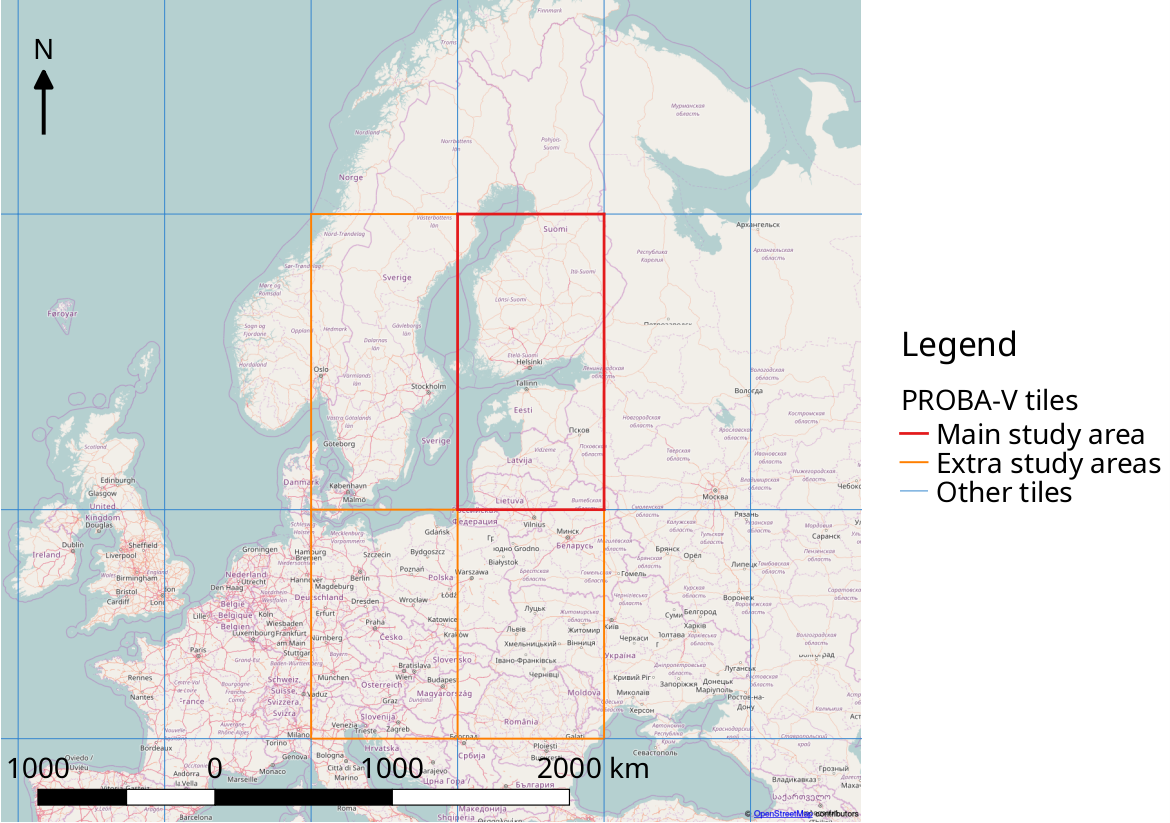
\includegraphics[width=\textwidth]{./proposal-figures/studyarea.png}
 \caption{Study area. The grid represents PROBA-V tiles (10 by 10 degree areas), tile 20,01 is highlighted in red, tiles 20,02, 19,01 and 19,02 are highlighted in orange.}
 \label{AOI}
\end{figure} 

The study area will be based on the PROBA-V tile 20,01. It spans from south Finland, known for boreal forests as well as a variety of lakes and boreal wetlands, to the middle of Lithuania, which includes both mixed and temperate broadleaf forests as well as protected wetlands. If time permits, tiles 20,02 (from middle of Lithuania to north of Bulgaria), 19,01 (south Sweden) and 19,02 (from north Poland and Germany to north Italy and Croatia) will also be used, by mosaicing them all into one large image (see figure \ref{AOI}).

The land cover classes that will be used for classification are based on the hybrid classification scheme by \citep{see2015hybrid}. The only change is the distinction between evergreen and deciduous tree cover (defined by whether the leaves have an annual senescence cycle or not). See table \ref{tbl-classes} for a full list.

\section{Ground truth data collection methods}

In order to make use of supervised classification algorithms, a representative dataset of ground truth at the area of interest has to be obtained for training the algorithms, as well as validating the classification accuracy. When working with fuzzy classification, the ground truth has to be in the same schema as the desired output from the classification algorithms. That means that every ground truth pixel has to contain information about the fraction of each class.

No such dataset was available at the time. The closest available was the Geo-Wiki Land Cover Classification Competition II result dataset. The participants of this competition were asked to identify up to three main land cover classes in a randomly selected 300 m resolution pixel and write down the class proportions. To do that, they had access to various satellite imagery and existing land cover classification maps. Each pixel could be validated by more than one person. While this dataset is close to what was needed for this study, several aspects made it unfit for use. First, within the area of interest, only 14 pixels were available. That is far from being enough, since classification algorithms need a representative sample of points for each class, of which in this study there were nine. Second, the contestants rarely agreed about the dominant classes and the proportions of each class in a pixel. Third, only up to three classes could be defined for each pixel, whereas all nine are required for this study. And fourth, the classification was based on a coarser resolution than the target in this study.

This meant that ground truth had to be collected manually specifically for the purposes of this study. Manual remote sensing image interpretation \citep{defries1998training} was used to achieve this. The target was to obtain at least 50 ground truth pixels for every class. A pixel was considered to belong to a certain class if that class had the majority fraction in the pixel. In addition, at least 15 pixels of each class had to be endmember pixels: ones that amount for 95\% or larger fractions within the pixel. The result was a dataset of 480 ground truth pixels in total.

For determining which pixels to sample, a two-stage selection protocol was used. The first stage was stratified random sampling based on the 2010 CCI Land Cover product by the European Space Agency. Since this product uses a larger number of classes (since it is a hard rather than a fuzzy classification), some classes were merged into one to fit the classes desired in this study. See table \ref{tbl-classes} for more details. 112 pixels per class (total of 1008) were selected in this stage.

\begin{table}
  \begin{center}
    \resizebox{\textwidth}{!}{
      \begin{tabular}{lp{9cm}l}
	\hline
	Class in this study & Equivalent classes in LC-CCI and their digital numbers & \\
	\hline
	\multirow{4}{*}{Crops} & Cropland rainfed & 10 \\
	  & Cropland rainfed - Herbaceous cover & 11 \\
	  & Cropland rainfed - Tree or shrub cover & 12 \\
	  & Cropland irrigated or post-flooding & 20 \\
	  & Mosaic cropland (>50\%) / natural vegetation (tree / shrub / herbaceous cover) (<50\%) & 30 \\
	\hline
	\multirow{7}{*}{Deciduous trees} & Tree cover  broadleaved  deciduous  closed to open (>15\%) & 60 \\
	  & Tree cover  broadleaved  deciduous  closed (>40\%) & 61 \\
	  & Tree cover  broadleaved  deciduous  open (15-40\%) & 62 \\
	  & Tree cover  needleleaved  deciduous  closed to open (>15\%) & 80 \\
	  & Tree cover  needleleaved  deciduous  closed (>40\%) & 81 \\
	  & Tree cover  needleleaved  deciduous  open (15-40\%) & 82 \\
	  & Tree cover  mixed leaf type (broadleaved and needleleaved) & 90 \\
	\hline
	\multirow{4}{*}{Evergreen trees} & Tree cover broadleaved evergreen closed to open (>15\%) & 50 \\
	  & Tree cover  needleleaved  evergreen  closed to open (>15\%) & 70 \\
	  & Tree cover  needleleaved  evergreen  closed (>40\%) & 71 \\
	  & Tree cover  needleleaved  evergreen  open (15-40\%) & 72 \\
	\hline
	\multirow{4}{*}{Shrubs} & Mosaic tree and shrub (>50\%) / herbaceous cover (<50\%) & 100 \\
	  & Shrubland & 120 \\
	  & Shrubland evergreen & 121 \\
	  & Shrubland deciduous & 122 \\
	\hline
	\multirow{4}{*}{Grass} & Grassland & 130 \\
	  & Lichens and mosses & 140 \\
	  & Mosaic herbaceous cover (>50\%) / tree and shrub (<50\%) & 110 \\
	  & Mosaic natural vegetation (tree/shrub/herbaceous cover) (>50\%) / cropland (<50\%) & 40 \\
	\hline
	\multirow{6}{*}{Bare soil} & Sparse vegetation (tree/shrub/herbaceous cover) (<15\%) & 150 \\
	  & Sparse shrub (<15\%) & 152 \\
	  & Sparse herbaceous cover (<15\%) & 153 \\
	  & Bare areas & 200 \\
	  & Consolidated bare areas & 201 \\
	  & Unconsolidated bare areas & 202 \\
	\hline
	\multirow{3}{*}{Wetland} & Tree cover flooded fresh or brakish water & 160 \\
	  & Tree cover flooded saline water & 170 \\
	  & Shrub or herbaceous cover flooded fresh/saline/brakish water & 180 \\
	\hline
	Urban & Urban areas & 190 \\
	\hline
	Water & Water bodies & 210 \\
	\hline
      \end{tabular}
    }
  \end{center}
  \caption{List of classes used in this study and their relation with LC-CCI classes. The LC-CCI classes listed for each class in this study were merged in order to perform stratified random sampling for the first stage of ground truth sample selection.}
  \label{tbl-classes}
\end{table}

The first stage selected pixels that were not always optimal for the needs of this study. First, endmember pixels were needed, while the vast majority of pixels are mixed. Second, the LC-CCI product uses coarser resolution pixels than the PROBA-V data used for classification, therefore the equivalent PROBA-V pixels were not necessarily of the desired land cover class. Third, LC-CCI classification was not always accurate, possibly due to inaccuracies in the classification algorithm used to derive it, and possibly due to land cover changes over time (PROBA-V data goes back only to 2013, three years later than what the LC-CCI product was made for). Fourth, the study requires ground truth where land cover types have remained constant over the last three years, wheras in some locations there was clear land cover change ocurring (mostly due to deforestation).

Therefore a systematic second stage selection was performed for each pixel selected in the first stage. Pixels within a 10 pixel radius from the first stage selection were manually checked, and the best pixel was selected for each. The first criterion considered was evident land cover change. No pixels with identifiable land cover change over the 2013-2016 period were used. The second criterion was uncertainty in identification of land cover fractions in the pixel. Pixels that had more unambiguous reference layers were preferred in order to minimise the uncertainty in the resulting dataset. The third criterion was the purity of the pixel. Pixels with one highly dominant land cover class were preferred, so that enough endmember pixels could be collected. The last criterion was the distance from the pixel selected in the first stage. In case all other criteria were equal for several pixels, the one closest to the pixel selected in the first stage was chosen. In case none of the pixels within the 10 pixel radius fulfilled the selection criteria, the area was skipped. In case the LC-CCI classification had mislabelled the area, a pixel of another class than the one desired could also be selected, provided it fulfills the above criteria. For example, the LC-CCI classification often confused urban and bare areas; in those cases, the best pixel was selected and identified appropriately, no matter which class it was labelled as in LC-CCI. See figure \ref{fig-sampling} for an example.

\begin{figure}
 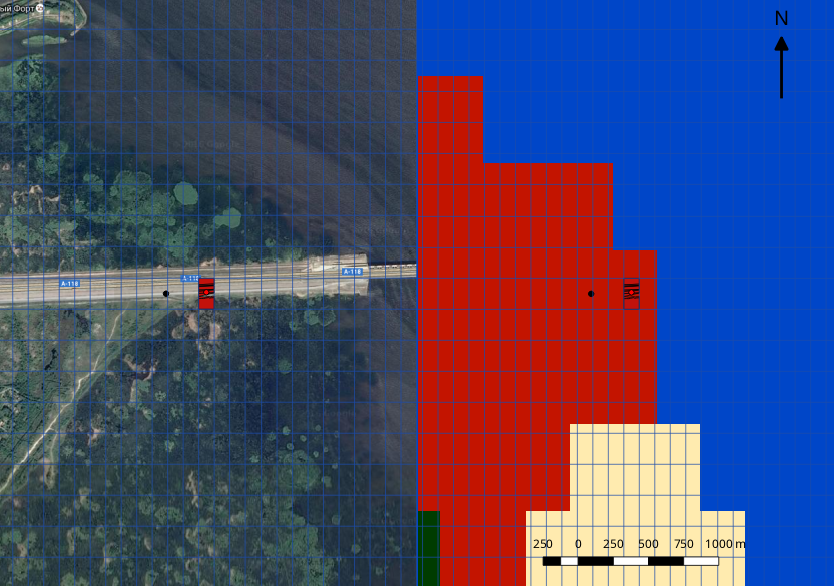
\includegraphics[width=\textwidth]{./thesis-figures/classification-example.png}
 \caption{An example of a ground truth pixel within an area misclassified by LC-CCI. Left: a true colour image of an area on Kotlin island, north of Kronstadt, Russia (Google Maps imagery). Right: LC-CCI classification of the same area. Red indicates urban areas, cream indicates sparsely vegetated areas, green indicates needleleaved evergreen forest. In reality, the area is mainly composed of wetland. The black point represents the first stage sample, the red point represents the second stage sample. The blue grid indicates PROBA-V pixel locations. The polygons around the second stage sample were used for measuring the area of each land cover type within the pixel. The result was 36\% wetland, 28\% urban, 23\% bare soil, 8\% grassland, 5\% shrubland, 0\% of the rest.}
 \label{fig-sampling}
\end{figure}

Image interpretation, second stage sample selection and dataset creation were performed using QGIS 2.14.8 ``Essen'' software. To aid in visual interpretation in order to ensure that the gathered ground truth would have as little uncertainty as possible, open national data (orthophotos and topographical maps) from Finland, Estonia, Latvia and Lithuania was used in addition to open global data. In addition to GIS layers, panoramic photos were used (Google Street View, Yandex panoramas). For a full list of layers used for image interpretation, see Appendix \ref{app-layerlist}.

In other to determine the class fractions within a PROBA-V pixel, instead of relying on subjective estimations or subdivision, land cover was outlined within a pixel by drawing multipart polygons for each class (except the dominant) on top of the parts of the pixel that represented the class. This takes extra time and effort, but results in more precise fraction measurements. Then by using a virtual attribute, the area of each polygon was calculated and divided by the total area of a pixel (which is constant among all pixels in the WGS84 coordinate reference system), giving a percentage fraction of each class. The fraction of the dominant class was then calculated by subtracting each of the other fractions from 100\%. Therefore the precision of the ground truth data is 1\% (ranging from 0\% to 100\%).

Gathered ground truth data was stored as a point layer, with each point describing the PROBA-V pixel under it. In order to make certain that there are no issues with points falling on pixel borders, as well as to accurately know the boundaries of each pixel when drawing polygons on it, a line grid was generated in QGIS by using an imported PROBA-V image as a reference for the origin and size of each grid cell. Ground truth points were placed in the centre of the pixel they describe, and snapping (with topology checking) was used when drawing polygons in order to avoid geometry errors and imprecisions.

The resulting sample points were then exported into a CSV file, which then was imported into R. Each attribute in R is available as a variable, so they can then be used in classification.

\section{Uncertainty considerations}

While care was taken to get reliable ground truth data, quite a few pixels chosen in the first selection stage had to be skipped due to too high uncertainty about the land cover fractions within the pixel, and there still exists a possibility of confusion between classes. Every class has its specifics.

First of all, while a large number of imagery sources were used to determine the land cover, their date of acquisition varies between different sources. Some of the sources, like Bing, do not give information about the year the image was taken. If land cover changes that affect the class fractions were identified, such pixels were not used as ground truth, but there exists a possibility that there had been land cover changes that were not identified due to the lack of recent imagery.

Another source of uncertainty comes from orthorectification of the imagery. Different sources were slightly offset from one another, in particular, Bing aerial imagery tended to be shifted around 16 metres from Google imagery of the same area in some places, and around 9 metres from national orthophoto imagery. When possible, Bing imagery was not used in favour of the other sources for drawing area measurement polygons. From those, the most recent or most detailed image was used.

Similarly, the look angle of the sensors tended to vary between images. That had most impact for tall objects, like tree canopies. Like with the point above, the most recent or finer resolution image was used as the main reference in that case. In addition, for deciduous trees, the season when the image was taken had an effect on the perception of tree canopies. In summer images, the canopy would seem to take up more area of the pixel than in images taken in other seasons. In order to cope with this problem, for images taken in other seasons, the polygons drawn on top of the trees were made larger to compensate, by estimating the area the canopy would take up if it was summer time.

Specifically for the crop class, there was a posibility of confusing it with the grass class for managed pastures. Crops were defined as managed herbaceous vegetation that is harvested at least once a year, thus pastures would rather fall into the grass class. But since pastures are also often managed, and there were not enough images to reliably detect whether at some point in the year the field is harvested, there may be confsing between the two. To mitigate this problem, panoramic images were used to identify cattle in the fields, whose presence would indicate whether the field is a pasture.

The distinction between evergreen and deciduous trees was also challenging. Within the study area, forests and stands primarily include trees of genus \textit{Betula} L. (birch trees), genus \textit{Pinus} L. (pine trees), of whom mostly \textit{Pinus sylvestris} L. (scots pine), and genus \textit{Picea} Mill. (spruce trees), of whom mostly \textit{Picea abies} (L.) H. Karst. (Norway spruce). Spruce canopies are distinctly conical, which allows distinguishing them from birch trees, but not from young pine trees. Also, very fine resolution imagery is required to tell the canopy shape in the first place. Such imagery was mostly available only in Estonia and parts of Finland. Distinguishing between birch trees and pine trees is even more challenging, since their canopy shape is very similar when looking from the top.

Two main approaches were used to deal with this source of uncertainty. The first approach was making use of imagery taken in seasons other than summer. In autumn, leaf senescence allows identifying deciduous trees directly by colour. In winter and spring, deciduous trees are difficult to discern from the forest floor, but by comparison with summer images, they show which areas consist of deciduous trees. In addition, such images reveal all evergreen trees within mixed forests. One pitfall of this approach could be that the changes in apparent tree cover between the images is not due to seasonality, but rather due to deforestation; however in practice, tree trunks are still visible in winter and spring imagery. With this approach, Estonian national imagery was most useful, since it was taken in late autumn and has a fine enough resolution to identify individual trees.

\begin{figure}
 \centering
 \subfloat[A sampled area in the town of Jyv\"askyl\"a, Finland.]
 {
  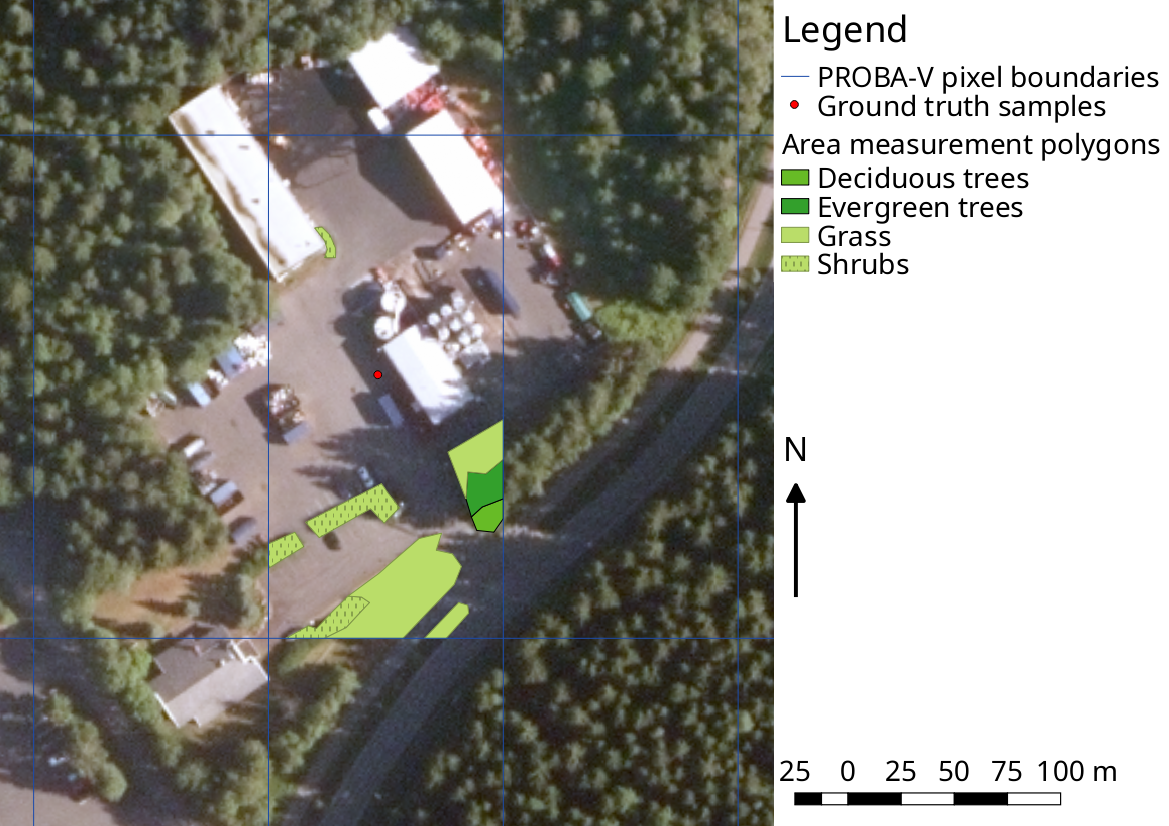
\includegraphics[width=\textwidth]{./thesis-figures/sample-example.png}
 }
 
 \subfloat[The same area in Google Maps, using 3D view.]
 {
  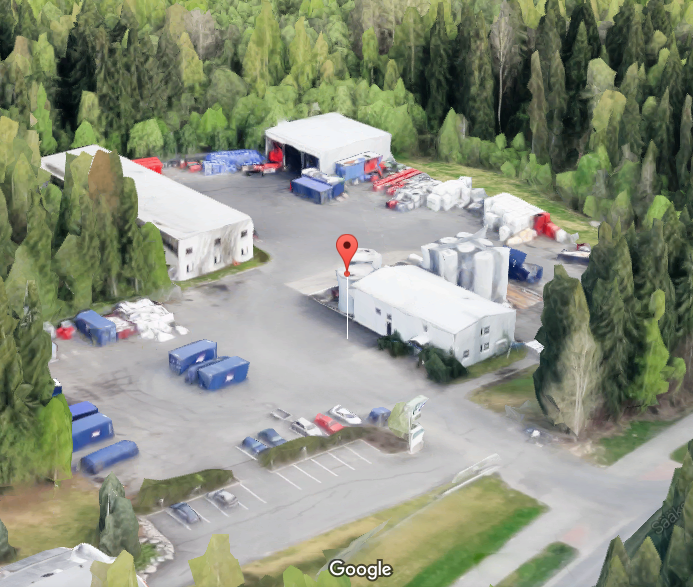
\includegraphics[width=0.8\textwidth]{./thesis-figures/sample-3d.png}
 }
 \caption{A close-up example of a sampled area for which 3D view was available for improved distinction between classes. The resulting land cover fractions were 87\% urban, 8\% grass, 3\% shrubs, 1\% evergreen trees, 1\% deciduous trees, 0\% others.}
 \label{fig-sampling-detailed}
\end{figure}

The second approach was to make use of auxiliary data. Most helpful were panoramic images, from which tree species could be identified directly. The limitation of this approach is that panoramic images are relatively scarce, limited to areas near roads. Also, typically only the first row of trees is visible in these images. But that is often enough to determine the proportion of deciduous and evergreen trees within a forest, and is useful when combined with remote sensing imagery, since by identifying the first tree row, further trees can be discerned by comparison. Another useful source of information were 3D models provided by Google Maps in certain areas. They are detailed enough to discern individual trees and their canopy shape, which allows identifying their type (see figure \ref{fig-sampling-detailed}). Other auxiliary data used were topographical maps, which sometimes marked forest types, and the LC-CCI classification map. Though this data was often not precise enough for the needs of this study. Lastly, in some images where the sun zenith angle was low, shadows could be used to determine the canopy shape of the first row of trees as well. But it was rather rare for this information to be useful, given the similarity in upper canopy between birch and pine trees.

Shrubs were problematic to distinguish between grass and both types of trees. Shrubs were defined as woody plants lower than 3 metres in height. That includes young trees and hedges, but does not include most low underwood species like apple trees \textit{Malus pumila} Mill. However, since most remote sensing imagery used was 2D, determining the height was problematic. One approach to distinguishing shrubs from trees was by comparison with other tree stands in the immediate vicinity. Since for most imagery the look angle was not equal to nadir, or there were shadows visible, comparing them with tree stands allows identification of this class. Another approach was once again to use panoramic photos in order to either identify the type of plants directly, or to estimate the height of the plants. The distinction between tall herbacious species (grass) and short woody species (shrubs) was also problematic at times. Panoramic photos were used in that case as well. Another consideration for this class is that within the area of interest, shrublands are a transitory ecosystem between grasslands and forests, they do not normally form a climax community. Similarly, young trees are transitory between grasslands (or, in case of reforestation, forest floor) and forests. In order to deal with this temporal aspect, all the available imagery was checked for differences of appearance between the images of different dates. If a patch of plants within a pixel appeared either as grass or as tall trees in any of the images, such a pixel was not used as a sample.

While bare soil was mostly easy to distinguish from the other classes, the specific case of roads lead to some uncertainty. Gravel roads were considered bare soil, while asphalt roads as well as roads made of concrete tiles were considered urban cover. In some of the imagery, the distinction of colour between the two was difficult to make, particularly in cases of eroded asphalt and asphalt covered by a thin layer of sand or dust. In those cases, panoramic photos were used to make a better distinction. Since there was a wealth of such photos taken on roads, this was for the most part a minor issue.

Wetlands were somewhat challenging to distinguish from grass and shrubs. This is by definition, since within the study area wetlands are covered by herbaceous or short woody vegetation. The distinguishing factor is whether the area is waterlogged or drained. However, this turned out to be a minor problem, because within the study area most wetlands are large, contiguous, often protected territories. They stand out, also by a more brown colour due to peat, from the surrounding environment at larger scales. Also, the LC-CCI map turned out to be rather accurate in detecting wetlands. Larger shrubs or young trees within wetlands were assigned to the shrub class. Another minor problem within wetlands was dealing with the seasonal change in herbaceous cover over the year, with plants taking up some area from open water in the summer. However, the changes were mostly small enough to not make a 1\% difference in the land cover fractions.

All in all there are many sources of uncertainty when it comes to image interpretation. Within this study most of them have been dealt with either by the sampling design (skipping uncertain pixels) or special considerations as mentioned above. It also helps improve accuracy that the ground truth is in fractions, so the actual position of the land cover within the pixel does not matter, and small errors may compensate one another. Still, it is inevitable that some of the gathered ground truth will not match the reality precisely.

\section{Model input data}

\subsection{Spectral data}
\label{sec-spectral}

PROBA-V sensor data was used for static, single-date spectral data. The 100 m spatial resultion top-of-canopy (TOC) data is provided in two varieties: one-day and five-day composites. The five-day composites are made by compositing five one-day composites by using maximum NDVI, after filtering out pixels of poor quality, such as incomplete data, sensor problems and extreme sun or look angles \citep{probavguide2}. However, even five-day composites are not enough to produce a fully cloud-free image of a single PROBA-V tile. Moreover, the cloud detection algorithm used for Collection 0 data is not suffient to fully detect all clouds. A reprocessing campaign using a more accurate algorithm that will result in Collection 1 data is ongoing \citep{probavguide2}, but the oldest images rather than the newest are being reprocessed first. At the moment of writing, the latest processed images are from the spring of 2015, which is not recent enough for the purposes of this study.

Therefore extra cloud masking and compositing was performed on the five-day composite data. A composite was created from the images of the whole summer of 2016 (2016-06-01 to 2016-08-31, 18 images in total). This was selected to minimise the effects of snow and senescence \citep{bartalev2014probavboreal}.

\subsection{Temporal data}

For deriving temporal data (vegetation growth phase, amplitude and period), a series of images spanning the entire lifetime of the PROBA-V mission (2013-2016, 3 years) will be used. The variables will be extracted by performing harmonic analysis \citep{rayner1971introduction,jakubauskas2001harmonic} on NDVI time series of the imagery.

\subsection{Auxiliary data}

Additional auxiliary data was also used in order to improve the classification accuracy. In particular, a digital elevation model (DEM) was used to derive elevation, slope, aspect and Topographic Position Index (TPI) terrain parameters. Such terrain parameters are known to increase the separability of vegetation classes \citep{burrough2001fuzzy}.

While the DEM from the NASA Global Land Survey (GLSDEM) was initially considered, since it has fine enough spatial resolution (3 arcseconds, approximately 90 m) and is already used by PROBA-V product suppliers for image ortho-rectification \citep{probavguide}. However, this DEM is in fact a combination of several DEMs, and in the study area above 60\textdegree{} latitude the DEM is based on GTOPO30 data that has 10 times coarser resolution (30 arcseconds, approximately a kilometre), resampled by using cubic convolution \citep{glsdemtechguide}. This makes it unsuitable for deriving slopes, since cubic convolution results in smoothed surfaces, whereas the original GTOPO30 data is of too coarse resolution compared to PROBA-V data.

Therefore the Digital Elevation Model over Europe (EU-DEM) by the European Environment Agency was used as a baseline DEM instead. It has 1-5 arcsecond (approx. 30-150 m) spatial resolution, achieved by fusing ASTER and SRTM satellite data, and covers all of the European Union countries \citep{bashfield2011eudem}. Since the study area also includes a parts of Belarus and a small part of Russia, GLSDEM was used to fill in the gaps there.

Slope was first calculated from the base DEM, using its native resolution and a 4-neighbour moving window, since the study area is mostly flat \citep{jones1998dem}. Afterwards, the values were resampled to PROBA-V pixels. This procedure results in more accurate representation of slopes compared to calculating them from resampled DEM data \citep{grohmann2015demresampling, wu2008demresampling}. Aspect was calculated from a resampled DEM instead, since it is angular data for which regular bilinear interpolation resampling technique does not apply. TPI, which is the difference between the height of a cell and the mean value of its 8 neighbours \citep{weiss2001topographic, wilson2007terrain}, was also calculated from resampled data due to stark differences in TPI between EU-DEM and GLSDEM datasets, which come from differences in spatial resolution (moving window size).

In addition to DEM-derived auxiliary data, vegetation indices derived from spectral data were also used, since a variety of vegetation indices are known to improve the separability of the wetlands class \citep{zhao2009indices,davranche2010wetland}. However, since the PROBA-V sensor only captures four spectral bands, the choice of available vegetation indices is limited. Therefore two vegetation indices that can be calculated and are known to improve wetlands separability were used: Optimised Soil-Adjusted Vegetation Index (OSAVI, \citealt{rondeaux1996osavi}) and Land Surface Water Index (LSWI, \citealt{xiao2004lswi}). These indices were calculated from the 2016 summer composite image as detailed in section \ref{sec-spectral}. While it is possible to use data from other sensors for deriving vegetation indices, attempting to match their pixels to those of PROBA-V would be bound to introduce inaccuracies due to resampling, thus that was not attempted.

\section{Classification algorithms}

There will be four classification algorithms tested in total: fuzzy c-means, fuzzy neural network, random forest regression and multiclass gradient boosting. All of these algorithms are available as packages for the \texttt{R} programming language. See table \ref{tbl-comparison} for a short comparison of the properties of the chosen algorithms.

\begin{table}
  \begin{center}
    \resizebox{\textwidth}{!}{
      \begin{tabular}{lllll}
	\hline
	Algorithm name & Supervised? & Fuzzy? & Single-model? & Type\\
	\hline
	Fuzzy c-means & Partially & Yes & Yes & Statistical\\
	Fuzzy neural network & Yes & Yes & Yes & Machine learning\\
	Random forest regression & Yes & Yes & No & Machine learning\\
	Multiclass gradient boosting & Yes & Partially & Yes & Machine learning\\
	\hline
      \end{tabular}
    }
  \end{center}
  \caption{Feature comparison between classification algorithms whose classification accuracy will be compared in the thesis. ``Partially fuzzy'' means the capability of training only on endmember pixels.}
  \label{tbl-comparison}
\end{table}

\subsection{Fuzzy c-means}

Fuzzy $c$-means, also called fuzzy $k$-means and supervised fuzzy $k$-means, is an algorithm based on the $k$-means clustering algorithm that attempts to classify pixels by identifying clusters by proximity in feature space. $k$-means is an unsupervised algorithm, and takes one parameter, $k$, for the number of clusters to create. These cluster centroids are usually selected randomly from all pixels, and clusters are formed by assigning each pixel to the class whose centre is the closest. Then the cluster centroids are recalculated, and the process is repeated until it converges. The supervised variety of this algorithm presets the cluster centroids to their known values from the training pixels, and the $c$-means or fuzzy $k$-means variety assigns each pixel a distance value from each class centroid to determine class membership. This makes the algorithm similar to maximum likelihood classification (it would be identical if the centroids were completely fixed). It also takes an extra parameter, called a fuzzification parameter, to determine the inverse of the distance from class centroids within which all pixels are said to belong exclusively to that class. A fuzzification parameter of 0 would result in hard classification, while a high value would make every pixel partially belong to all classes. \citep{hengl2004fuzzycmeans}

The advantage of this algorithm is its simplicity: increasing the number of pixels should not result in high increase in processing time, as only the points' centroid and the distance from each class centroid to each pixel has to be calculated. The disadvantage is that it is only partially supervised, very little data from the training pixels are used (only the class centroid position from a weighted average).

\subsection{Fuzzy neural network}

Neural networks are a machine learning algorithm that works by making use of a layered architecture of an input layer, output layer, and a number of hidden layers in between. When training, the algorithm tries to assign weights to each node in the hidden layers so that given the input layer, the result would be the output layer. Initially values are assigned at random, and by using a back-propagation algorithm they are adjusted to better fit the output. Such a trained neural network can then predict the output layer values when given unclassified pixels as the input layer. \citep{foody1997fuzzynnet}

Neural networks work with continuous values, therefore they can take mixed pixels as training input, and output continuous membership values for every class, which makes them well-suited for fuzzy classification tasks. However, the downside of neural network is that they require three parameters: the number of hidden layers, the number of neurons (nodes) per each hidden layer, and the number of back-propagation iterations. Each of these affect the ability of the neural network to generalise data instead of overfitting the training output, and there is no rule of thumb about what combination should work the best, requiring a lot of trial and error or Monte Carlo analysis to get satisfactory results.

\subsection{Random forest}

Random forest is another machine learning algorithm, based on building decision trees that could be used to determine the class of a pixel. The algorithm generates a (configurably) large number of decision trees, each based on a random (with replacement) training subsample, so that every tree in the model is unique. Then in order to determine which class a pixel belongs to, each tree casts a vote. With hard classification, the pixel is assigned the class with the majority vote. \citep{walton2008subpixelrf}

With fuzzy classification, instead of using the majority vote, the fraction of votes can be used as an indication of class membership instead. However, the algorithm will have to be trained on endmember pixels only in that case. Alternatively, random forest is also capable of performing regressions, but only for single output variables. Thus by performing one regression for each class (binary relevance method), mixed pixels could be used for training, but the algorithm will not take other classes into account.

\subsection{Gradient boosting}

Gradient boosting is a machine learning algorithm highly related to random forest. The difference is that instead of building random trees and having them vote, the algorithm iteratively optimises a tree (or a small set of trees) to better fit the training data, while making sure not to add unnecessary complexity to the model by performing internal cross-validation at each step. Much like the two aforementioned machine learning methods, it internally uses continuous values, and the result can be expressed as a sum of all tree branch weights. \citep{friedman2001gradientboost}

Just like with random forest, there are two ways to use this algorithm for fuzzy classification: the binary relevance method, or a multiclass method that gives the probability of a pixel to belong to each class, akin to the random forest vote fraction method. The same advantages and disadvantages apply.

\section{Validation and visualisation}

In order to perform validation on the classification results, validation metrics that work on fuzzy classification are needed. While there are several approaches, the metrics that are easiest to interpret and that are most often used for this purpose are based on the well-known statistical concept of error (also referred to as distance in some literature) \citep{foody1996fuzzyevaluation}. In particular, the mean absolute error (MAE) and root mean square error (RMSE) for every class will be used to assess classification accuracy in this thesis. The validation will be performed by splitting the ground truth samples into a training and a validation set. For algorithms that can handle mixed pixel training data, 4-fold cross-validation will be used to split the data. For algorithms that cannot, all endmember pixels will be used as the training set and all mixed pixels will be used as the validation set. The training set will be used to train the classification algorithms, and the validation set will be used to determine the accuracy of the algorithm predictions by:

$$ RMSE_c = \sqrt{ \displaystyle\sum_{i=1}^{n}{ (p_{i} - v_{i})^2 } \over{n} } $$

where $ RMSE_c $ is the root mean squared error of class $ c $, $ v_{i} $ is the true degree of $ i $th pixel's membership to class $ c $ (in percent), $ p_i $ is the predicted degree of $ i $th pixel's membership to class $ c $, and $ n $ is the total number of pixels in an image, and

$$ MAE_c = {\displaystyle\sum_{i=1}^{n}{ |p_{i} - v_{i}| } \over{n}} $$

where $ MAE_c $ is the mean absolute error of class $ c $.

These two statistics show how many percent did the algorithm either overrepresent or underrepresent class $ c $ membership of all pixels in the image on average. The difference between the two is that RMSE gives a larger penalty for large errors compared to MAE.

These statistics allow comparing how the algorithm is capable of separating each class, much like a confusion matrix does in hard classification. A difference is that this approach does not give information about which classes the algorithm has trouble separating (as it is also a matter of degree in fuzzy classification). A total classification accuracy statistic can be obtained by taking a mean of all class RMSE and MAE statistics.

In addition to accuracy statistics, a bias statistic mean error (ME) will also be calculated for each class:

$$ ME_c = {\displaystyle\sum_{i=1}^{n}{ (p_{i} - v_{i}) } \over{n}} $$

Positive ME values mean that the algorithm tends to overrepresent class $c$ membership, negative ME values mean that it tends to underrepresent class $c$ membership on average in all pixels. An ME of 0 would mean that the algorithm is unbiased.

\bibliography{bibliography}

\begin{appendices}
 \chapter{Visual interpretation layers}
 \label{app-layerlist}
 \begin{table}
  \begin{center}
    \resizebox{\textwidth}{!}{
      \begin{tabular}{llrl}
	\hline
	Layer provider & Layer type & Year & URL \\
	\hline
	ESA LC-CCI & Land cover & 2010 & \url{http://maps.elie.ucl.ac.be/CCI/viewer} \\
	OpenStreetMap & Topographical & 2016 & \url{http://www.openstreetmap.org} \\
	Google & Satellite & ?-2016 & \url{https://www.google.com/maps} \\
	Google & Panoramic & 2009-2016 & \url{https://www.google.com/maps} \\
	Bing & Satellite & ?-2016 & \url{https://www.bing.com/maps} \\
	Yandex & Satellite & ?-2016 & \url{https://yandex.com/maps/} \\
	Yandex & Panoramic & ?-2016 & \url{https://yandex.com/maps/} \\
	Lithuania & Topographical & 2016 & \url{http://www.geoportal.lt} \\
	Lithuania & Orthophoto & 2005-2015 & \url{http://www.geoportal.lt} \\
	Latvia & Orthophoto & 2010-2011 & \url{http://www.lgia.gov.lv} \\
	Latvia & Orthophoto & 2010 & \url{http://www.gisnet.lv/cgi-bin/osm_latvia} \\
	Estonia & Topographical & 2016 & \url{http://geoportaal.maaamet.ee} \\
	Estonia & Orthophoto & 2007-2009 & \url{http://geoportaal.maaamet.ee} \\
	Finland & Topographical & 2016 & \url{http://kartat.kapsi.fi} \\
	Finland & Orthophoto & 2006-2016 & \url{http://kartat.kapsi.fi} \\
	\hline
      \end{tabular}
    }
  \end{center}
  \caption{List of layers used to aid visual interpretation when gathering ground truth data. Most of the layers were accessed as WMS or TMS services (exceptions: Google Street View and Yandex accessed through a web interface; Google and Bing satellite data accessed using JavaScript API).}
  \label{tbl-layers}
\end{table}
\end{appendices}

\end{document}

%Training: Forest + grass + urban + water ~ Blue + Red + NIR + SWIR + Period + Phase + Amplitude + Etc
%To predict: . ~ Blue + Red + NIR + SWIR + Period + Phase + Amplitude + Etc
